% ============================================================================
% Isaac Kobby Anni — Preliminary Report (LaTeX Template)
% Mirrors the format you shared, keeping structure/styles intact.
% Fill in the placeholders after you share the papers; I’ll help populate.
% ============================================================================
\documentclass{article}

% ----- Packages (kept to match original style) -----
\usepackage{amsmath, amsthm, amssymb, amsfonts, mathtools}
\usepackage{thmtools}
\usepackage{graphicx}
\usepackage{setspace}
\usepackage{geometry}
\usepackage{float}
\usepackage{hyperref}
\usepackage[utf8]{inputenc}
\usepackage[english]{babel}
\usepackage{framed}
\usepackage[dvipsnames]{xcolor}
\usepackage{tcolorbox}
\usepackage{enumitem}
\usepackage{multirow}
\usepackage{natbib}
\usepackage[table,xcdraw]{xcolor}
\hypersetup{pdfborder = {0 0 0}}

% ----- Colors & utilities (kept from original) -----
\colorlet{LightGray}{White!90!Periwinkle}
\colorlet{LightOrange}{Orange!15}
\colorlet{LightGreen}{Green!15}

\newcommand{\HRule}[1]{\rule{\linewidth}{#1}}
\newcommand{\disp}{\displaystyle}

% ----- Theorem-like envs with tcolorbox (kept) -----
\declaretheoremstyle[name=Theorem,]{thmsty}
\declaretheorem[style=thmsty,numberwithin=section]{theorem}
\tcolorboxenvironment{theorem}{colback=LightGray}

\declaretheoremstyle[name=Proposition,]{prosty}
\declaretheorem[style=prosty,numberlike=theorem]{proposition}
\tcolorboxenvironment{proposition}{colback=LightOrange}

\declaretheoremstyle[name=Principle,]{prcpsty}
\declaretheorem[style=prcpsty,numberlike=theorem]{principle}
\tcolorboxenvironment{principle}{colback=LightGreen}

\setstretch{1.2}
\geometry{margin=1.0in}

% ----- Meta (edit these) -----
\newcommand{\studentName}{Isaac Kobby Anni}
\newcommand{\department}{Department of Computer Science}
\newcommand{\reportTitle}{Preliminary Report — Critical Reviews of Selected Papers}
\newcommand{\committee}{\textbf{Prelim Committee:} \\ Dr. Md Main Uddin Rony, Chair \\ Prof. Dasigi \\ Prof. Robert Green \\ Dr. Umar Islambekov \\ Dr. Sara Slitter}
\newcommand{\degreeContext}{Ph.D. Preliminary Examination}

% ----- Helper Macros -----
% Use these to stamp each reviewed paper cleanly.
\newcommand{\PaperHeader}[3]{%
  \section{#1} % Paper Title as section
  \noindent\textbf{Authors:} #2\\
  \textbf{Venue/Year:} #3\\[4pt]
  % Optional link
  % \textbf{URL:} \url{https://...}
  \vspace{0.5em}\hrule\vspace{1em}
}

% ============================================================================
\begin{document}

% ----- Cover -----
\title{\normalsize \textsc{\degreeContext}\\[2.0cm]
  \HRule{1.5pt} \\
  \LARGE \textbf{\uppercase{\reportTitle}}\\
  \HRule{2.0pt} \\[0.6cm]
  \LARGE{\\Reviewed and Prepared by \\
  \studentName} \vspace*{7\baselineskip}}

\date{\today}
\author{\department}
\maketitle
\vspace*{1em}
\committee

\newpage
\tableofcontents
\newpage

% ============================================================================
% 0. Introduction (kept structure & tone from original)
% ============================================================================
\section{Introduction}
The rapid evolution of agentic artificial intelligence systems presents both unprecedented opportunities and significant challenges for deploying efficient, cost-effective, and privacy-preserving AI agents at scale. As the field transitions from proof-of-concept demonstrations to production-ready systems, fundamental questions emerge about optimal architectural choices, resource allocation, and deployment strategies that can enable widespread adoption while maintaining performance standards. \\\\
This preliminary report examines three pivotal papers that collectively address critical aspects of agentic AI development: automated feature engineering through language model interfaces, the economic and operational advantages of small language models in agentic systems, and scalable training strategies that enable efficient model development. These works represent distinct yet complementary perspectives on how to build practical, deployable agentic systems that balance capability, efficiency, and cost.\\\\
For each paper, I provide a comprehensive analysis that (i) summarizes core contributions and novel insights, (ii) formalizes the problem setting and underlying assumptions, (iii) details the methodology with appropriate notation and mathematical frameworks, (iv) examines empirical results and their implications, (v) offers critical appraisal and positions the work relative to alternative approaches, and (vi) connects the paper's insights to my dissertation research on small language model deployment for privacy-sensitive agentic applications.\\\\
The synthesis of these papers informs my research agenda focused on developing SLM-first agentic architectures that can operate efficiently in edge computing environments while maintaining performance standards. This work contributes to the broader goal of democratizing access to advanced AI capabilities through more efficient and accessible deployment paradigms.


% ============================================================================
% Paper 1
% ============================================================================
\PaperHeader{Large Language Models for Automated Data Science: Introducing CAAFE for Context-Aware Automated Feature Engineering}{Noah Hollmann; Samuel Müller; Frank Hutter}{NeurIPS 2023} \citep{hollmann2023large}

\subsection{Problem Setup and Motivation}
While automated machine learning (AutoML) has achieved remarkable success in optimizing the machine learning pipeline, it remains largely ineffective at addressing the most time-consuming aspect of data science: data engineering and feature construction. According to industry surveys, model selection, training, and scoring account for only 23\% of a data scientist's time, leaving the majority of effort focused on data preparation and feature engineering tasks that require domain expertise and contextual understanding. \\\\
The authors identify a critical gap in current AutoML systems: the inability to incorporate semantic and contextual information into automated feature engineering processes. Traditional approaches like Deep Feature Synthesis (DFS) and AutoFeat rely on mathematical transformations and combinatorial exploration of feature spaces, but lack the ability to leverage domain knowledge that human experts naturally apply when engineering features.\\\\
CAAFE addresses this limitation by proposing a novel paradigm that bridges the semantic understanding capabilities of large language models with the robustness and interpretability of classical machine learning algorithms. The approach leverages LLMs' extensive domain knowledge to generate contextually meaningful features while maintaining the reliability of traditional ML validation methods.
\begin{figure}[H]
  \centering
  \includegraphics[width=0.95\linewidth]{img/context_benefit.png}
  \caption{Contextual information can simplify a task immensely. On the left-hand side no contextual information is added to the plot, and it is hard to predict the label for the green query point. On the right-hand side contextual information is added and a useful additional feature (weekend or weekday) is derived from which a mapping from features to targets can be found}
\end{figure}

\subsection{Formal Framework and Assumptions}
CAAFE operates within a formal framework that combines iterative feature generation with performance-based validation. Given training and validation datasets $(D_{\text{train}}, D_{\text{valid}})$ and a textual context description $c$, the method follows a structured iterative process:\\\\
\textbf{Input Components:} The system requires (1) dataset metadata including feature names, data types, and missing value statistics, (2) a user-provided contextual description of the domain and task, (3) sample data rows to provide scale and encoding information, and (4) a template specifying the expected output format for generated code.\\\\
\textbf{Iterative Process:} Each iteration $t$ follows the sequence: (1) construct a comprehensive prompt incorporating dataset context and previous iteration feedback, (2) generate Python code block $\phi_t$ and natural language justification via LLM, (3) execute code safely on current datasets to produce $D'_{\text{train}}$ and $D'_{\text{valid}}$, (4) evaluate performance $P'_t$ using cross-validation, (5) accept feature if $P'_t > P_{t-1}$, otherwise reject and maintain previous state.\\\\
\textbf{Key Assumptions:} The framework assumes (1) safe code execution environment with whitelisted operations, (2) deterministic evaluation procedures, (3) stable baseline learner performance, (4) meaningful contextual descriptions, and (5) sufficient computational resources for iterative evaluation.

\subsection{Methodology}

\subsubsection{Prompt Engineering and Code Generation}
CAAFE employs sophisticated prompt engineering to guide LLM behavior toward generating semantically meaningful features. The prompt construction process incorporates multiple components:\\\\
\textbf{Contextual Information:} User-generated dataset descriptions provide domain-specific context that guides feature generation toward relevant transformations. This includes task descriptions, domain knowledge, and specific requirements for the prediction task.\\\\
\textbf{Technical Specifications:} The prompt includes feature names with semantic meaning, data types (float, int, category, string), missing value percentages, and sample data rows that provide insight into data encoding and scale.\\\\
\textbf{Template Structure:} A standardized template guides the LLM to produce code that follows a specific format: feature name, usefulness explanation, input feature identification, sample value analysis, and executable Python code using pandas operations.\\\\
\textbf{Chain-of-Thought Instructions:} The system employs reasoning step instructions that encourage the LLM to explicitly consider the high-level meaning of generated features, identify relevant input features, analyze sample values, and then construct appropriate code transformations.
\subsubsection{Safety and Error Handling}
The methodology incorporates several safety mechanisms to ensure reliable operation:\\\\
\textbf{Code Execution Safety:} Generated Python code is executed within a restricted environment that whitelists only safe operations. Imports, arbitrary function calls, and potentially dangerous operations are excluded from execution.\\\\
\textbf{Error Recovery:} When code execution fails, error messages are fed back to the LLM in subsequent iterations, enabling automatic recovery and correction of invalid code. This feedback loop allows the system to learn from execution failures and generate corrected implementations.\\\\
\textbf{Resource Management:} While not providing complete security, the system attempts to prevent infinite loops and excessive resource usage through careful prompt engineering and execution monitoring.

\begin{figure}[H]
  \centering
  \includegraphics[width=0.95\linewidth]{img/caafe_workflow.png}
  \caption{CAAFE iterative workflow: Context specification leads to LLM-generated feature engineering code, which is executed and validated against performance metrics. Only improvements are retained, creating a self-improving feature engineering pipeline.}
\end{figure}

\subsubsection{Evaluation and Validation}
The validation methodology employs rigorous performance assessment:\\\\
\textbf{Cross-Validation Protocol:} Each feature is evaluated using ten random validation splits with consistent train/test proportions. Performance is measured using both accuracy and ROC AUC metrics, with mean improvement across both metrics determining feature acceptance.\\\\
\textbf{Baseline Comparison:} Features are accepted only when they demonstrate improvement over the current best performance, ensuring that the iterative process maintains or improves model quality.\\\\
\textbf{Computational Efficiency:} The system uses TabPFN for rapid feature evaluation, enabling efficient iteration through multiple feature proposals while maintaining reliable performance assessment.

\subsection{Experiments / Evidence}

\subsubsection{Performance Results}
CAAFE demonstrates substantial performance improvements across diverse tabular datasets. The primary evaluation uses TabPFN as the downstream classifier, with CAAFE improving performance on 11 out of 14 datasets. The mean ROC AUC improvement from 0.798 to 0.822 represents a significant enhancement comparable to switching from logistic regression to random forest on the same datasets.\\\\
\textbf{Dataset Diversity:} The evaluation spans both established benchmarks from OpenML (released before September 2021) and newer datasets from Kaggle (released after the LLM training cutoff), ensuring that improvements are not due to training data contamination.\\\\
\textbf{Classifier Generalization:} Results demonstrate consistent improvements across multiple downstream classifiers including logistic regression, random forests, and state-of-the-art methods like AutoGluon, indicating that CAAFE's benefits are not specific to particular model architectures.\\\\
\textbf{Feature Engineering Synergy:} When combined with traditional automated feature engineering methods like DFS and AutoFeat, CAAFE provides additional benefits for less powerful classifiers while maintaining advantages for sophisticated methods like TabPFN.

\subsubsection{Feature Generation Patterns}
Analysis of generated features reveals several common strategies employed by CAAFE:\\\\
\textbf{Feature Combination:} The system frequently generates features that combine multiple input variables, such as creating interaction terms or logical combinations that capture domain-specific relationships.\\\\
\textbf{Discretization and Binning:} Numerical features are often transformed into categorical representations through intelligent binning strategies that reflect domain knowledge about meaningful thresholds.\\\\
\textbf{String Processing:} Textual features undergo sophisticated parsing and extraction operations, such as extracting deck information from cabin codes or identifying patterns in structured text data.\\\\
\textbf{Feature Selection:} The system demonstrates the ability to identify and remove redundant features when newly generated features capture the same information more effectively.
\subsubsection{Error Recovery and Robustness}
CAAFE exhibits remarkable resilience to code generation errors, with only 7.4\% of generated features requiring error recovery across all experimental runs. The feedback mechanism successfully enables the system to correct issues such as missing value handling, type conversion errors, and logical inconsistencies in generated code.

\subsection{Strengths, Limitations, and Edge Cases}
\textbf{Strengths:} CAAFE's primary advantages include its ability to generate interpretable features with human-readable explanations, its scalability through code-based transformations that apply to entire datasets, and its robustness through classical ML validation methods. The system successfully bridges the gap between LLM semantic understanding and traditional ML reliability.\\\\
\textbf{Limitations:} The approach depends heavily on prompt quality and user-provided context descriptions. The evaluation methodology lacks statistical significance testing, and the system may plateau when baseline learners cannot express the nonlinearities captured by generated features. Computational overhead increases with the number of feature proposals evaluated.\\\\
\textbf{Edge Cases:} The method faces challenges with datasets containing large numbers of features, which can create prompts that exceed LLM processing capabilities. The reliance on LLM hallucinations for feature generation may produce seemingly logical but ultimately ungrounded features. The statistical validation approach could be improved through more sophisticated hypothesis testing.

\subsection{Connections to My Dissertation}
This work provides crucial insights for my research on SLM-first agentic architectures, particularly in the context of automated data science workflows. The "code-as-interface" paradigm demonstrated by CAAFE aligns perfectly with my proposed framework for deploying small language models in privacy-sensitive environments.\\\\
\textbf{SLM Integration Potential:} The iterative feature engineering process could be efficiently implemented using specialized SLMs trained for code generation tasks, reducing computational costs while maintaining the semantic understanding necessary for effective feature engineering. The structured prompt engineering approach provides a template for designing SLM-specific prompts that maximize performance within constrained parameter budgets.\\\\
\textbf{Privacy-Preserving Applications:} CAAFE's approach enables feature engineering without exposing sensitive data to external LLM services. Local SLM deployment could generate candidate features while maintaining data privacy and reducing operational costs.\\\\
\textbf{Validation Framework:} The performance-based validation methodology provides a robust framework for evaluating SLM-generated features in agentic systems, ensuring that automated feature engineering maintains quality standards while operating within resource constraints.

\subsection{Key Takeaways}
CAAFE establishes several critical insights for the future of automated data science: (1) Language-to-code agency provides a viable pathway for incorporating semantic understanding into automated feature engineering, (2) Iterative validation with performance metrics creates a natural safety mechanism that ensures continuous improvement, (3) The modular architecture enables seamless integration with existing AutoML pipelines, and (4) The approach demonstrates the potential for SLM deployment in specialized feature engineering tasks, offering a path toward more efficient and privacy-preserving automated data science workflows.

% ============================================================================
% Paper 2
% ============================================================================
\PaperHeader{Small Language Models are the Future of Agentic AI}{Peter Belcak; Greg Heinrich; Shizhe Diao; Yonggan Fu; Xin Dong; Saurav Muralidharan; Yingyan Celine Lin; Pavlo Molchanov}{NVIDIA Research, 2025 (preprint)} \cite{belcak2025small}

\subsection{Problem Setup and Motivation}
The agentic AI landscape has experienced explosive growth, with over half of large IT enterprises actively deploying AI agents and the sector reaching \$5.2 billion in market valuation with projections to \$200 billion by 2034. However, this rapid adoption has been predicated on a potentially misaligned architectural choice: the pervasive use of large language models (LLMs) for tasks that may not require their full generality and computational overhead.\\\\
The authors present a compelling counter-narrative to the current industry standard. Rather than viewing agentic systems as applications requiring the broad conversational capabilities and extensive world knowledge of LLMs, they argue that most agentic workflows decompose complex goals into modular, repetitive subtasks that are inherently narrow in scope. These subtasks—tool calling, data extraction, format transformation, and structured reasoning—demand precision and efficiency rather than conversational fluency. The paper challenges the fundamental assumption that LLMs are the optimal choice for such constrained environments and proposes a paradigm shift toward small language models (SLMs) as the primary drivers of agentic intelligence.

\subsection{Formal Framework and Assumptions}
The authors establish clear working definitions to ground their position: SLMs are language models that can operate on consumer-grade hardware with latency sufficient for real-time user interaction, while LLMs are defined simply as models that do not meet the SLM criteria. As of 2025, this translates to models with fewer than 10 billion parameters qualifying as SLMs.\\\\
The framework evaluates three core dimensions: \textbf{capability sufficiency} (whether SLMs can handle agentic subtasks), \textbf{operational suitability} (architectural advantages for agentic deployment), and \textbf{economic viability} (cost-benefit analysis of SLM versus LLM deployment). The analysis considers both homogeneous systems (single model type) and heterogeneous architectures that strategically combine SLMs and LLMs based on task complexity.\\\\
The position rests on several key assumptions: (1) agentic systems can be decomposed into specialized subtasks, (2) most agentic interactions are deterministic rather than conversational, (3) infrastructure costs scale with model size and deployment complexity, and (4) the current scaling laws for language models may not apply uniformly across all task domains.

\subsection{Methodology (Position Arguments)}

\subsubsection{Capability Sufficiency Argument}
The paper presents extensive evidence that modern SLMs have reached capability parity with much larger predecessors on agentic-relevant tasks. Microsoft's Phi-2 (2.7B parameters) achieves commonsense reasoning and code generation scores comparable to 30B models while operating 15× faster. The Phi-3 small (7B) demonstrates language understanding on par with 70B models of the same generation. NVIDIA's Nemotron-H family (2-9B parameters) achieves instruction following and code generation accuracy comparable to dense 30B LLMs at an order-of-magnitude reduction in inference FLOPs.\\\\
These examples illustrate a broader trend: capability gaps between SLMs and LLMs are narrowing rapidly, particularly in structured tasks like tool calling and instruction following. The authors argue that for agentic applications, raw parameter count is less predictive of performance than task-specific optimization and appropriate architectural choices.

\subsubsection{Economic Viability Analysis}
The economic argument centers on three factors: inference efficiency, fine-tuning agility, and deployment flexibility. Serving a 7B SLM costs 10-30× less than a 70-175B LLM in terms of latency, energy consumption, and computational requirements. This efficiency enables real-time agentic responses at scale while dramatically reducing operational costs.\\\\
Fine-tuning represents another critical advantage. Parameter-efficient techniques like LoRA and DoRA allow SLMs to be specialized for specific agentic tasks in hours rather than weeks, enabling rapid adaptation to changing requirements. The smaller model size also facilitates edge deployment, as demonstrated by systems like ChatRTX that enable local execution on consumer-grade GPUs.

\subsubsection{Operational Architecture Considerations}
The paper identifies two primary architectural patterns for agentic systems:

\begin{figure}[H]
  \centering
  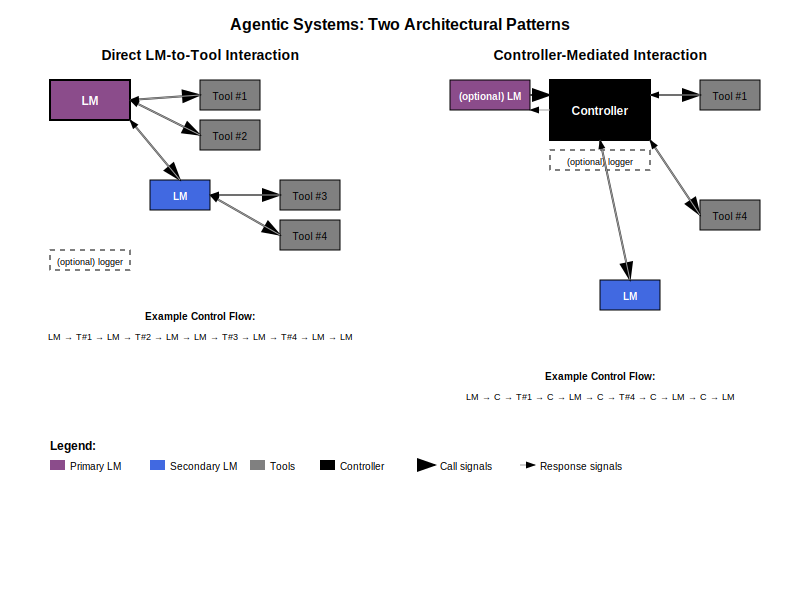
\includegraphics[width=17cm, height = 6cm]{img/agentic_architectures.png}
  \caption{Two distinct architectural patterns for agentic AI systems. Left: Direct LM-to-Tool Interaction where language models directly orchestrate tool calls. Right: Controller-Mediated Interaction where a dedicated controller manages all LM-tool interactions.}
\end{figure}

\paragraph{Direct LM-to-Tool Interaction:} In this model, the language model serves both as the human-computer interface and the primary orchestrator of tool calls. The LM directly manages interactions with tools and can delegate to other specialized LMs as needed. This approach offers maximum flexibility but requires careful prompt engineering and error handling.\\\\
\textbf{Controller-Mediated Interaction:} Here, a dedicated controller code manages all interactions between LMs and tools. The controller can route requests to specialized SLMs for different subtasks while maintaining centralized logging and error handling. This architecture enables more predictable behavior and easier debugging but may introduce additional latency.\\
Both architectures support heterogeneous model deployment, allowing agents to use SLMs for routine tasks while escalating to LLMs only when broader reasoning or conversational capabilities are required.

\subsection{Experiments / Evidence}
While this is fundamentally a position paper, the authors provide substantial empirical evidence through comprehensive benchmarking of recent SLM families. The analysis covers multiple dimensions: commonsense reasoning (indicating basic understanding), tool calling and code generation (measuring interface communication abilities), and instruction following (assessing response quality).\\\\
Notable examples include DeepSeek-R1-Distill models (1.5-8B parameters) that outperform proprietary models like Claude-3.5-Sonnet and GPT-4o on commonsense reasoning. Salesforce's xLAM-2-8B achieves state-of-the-art performance on tool calling despite its modest size. These results suggest that well-designed SLMs can compete with frontier models on specific agentic tasks.\\\\
The paper also outlines a practical LLM-to-SLM conversion algorithm involving usage data collection, task clustering, specialized fine-tuning, and iterative refinement. This provides a concrete pathway for organizations to transition from LLM-centric to SLM-first agentic architectures.

\subsection{Strengths, Limitations, and Edge Cases}
\textbf{Strengths:} The paper presents a compelling economic and operational argument grounded in real performance data. The heterogeneous architecture approach acknowledges that some tasks may still require LLM capabilities while optimizing for the majority of agentic subtasks. The conversion algorithm provides practical guidance for implementation.

\paragraph{Limitations:} The empirical evidence relies heavily on external benchmarks rather than end-to-end agentic system evaluations. Some agentic tasks may require world knowledge breadth or long-horizon reasoning that current SLMs may not adequately capture. The analysis focuses primarily on technical capabilities while giving less attention to safety and alignment considerations in edge deployment scenarios.

\paragraph{Edge Cases:} The paper acknowledges that certain agentic applications may still require LLM capabilities, particularly those involving open-domain dialogue, complex multi-step reasoning, or tasks requiring extensive world knowledge. The proposed solution is heterogeneous systems that can gracefully handle such cases through intelligent routing.

\subsection{Connections to My Dissertation}
This work directly supports my \emph{SLM-first} research agenda by providing both theoretical justification and practical implementation guidance. The heterogeneous architecture approach aligns with my proposed edge computing framework for efficient and privacy-preserving agentic systems.\\\\
The economic analysis validates my hypothesis that SLM deployment can achieve significant cost reductions while maintaining task performance. The conversion algorithm provides a concrete methodology for transitioning existing LLM-based systems to more efficient SLM architectures.\\\\
The architectural patterns discussed in the paper inform my planned agent designs, particularly the controller-mediated approach for ensuring predictable behavior in sensitive environments. The emphasis on task decomposition and specialized fine-tuning resonates with my research on domain-adaptive SLMs for specific application contexts.
\begin{figure}[H]
  \centering
  \includegraphics[width=0.95\linewidth]{img/controller.png}
  \caption{Left: a single large LLM plans, routes, and answers end-to-end—simple, but high cost/latency and limited control. Right (proposed): a lightweight controller routes subtasks to specialized SLMs and tools, then synthesizes the result—lower cost/latency, better observability/debugging, and feasible on consumer-grade hardware.}
\end{figure}

\subsection{Key Takeaways}
The paper makes a compelling case for reconsidering the default choice of LLMs in agentic systems. The key insights are: (1) capability gaps between SLMs and LLMs are narrowing rapidly for agentic-relevant tasks, (2) economic advantages of SLMs are substantial and will likely increase as infrastructure costs continue to fall, (3) heterogeneous architectures provide a practical path forward that preserves LLM capabilities where needed while optimizing for efficiency elsewhere, and (4) the industry's current LLM-centric approach may represent a suboptimal allocation of computational resources that could be addressed through systematic migration to SLM-first designs.


% ============================================================================
% Paper 3
% ============================================================================
\PaperHeader{MiniCPM: Unveiling the Potential of Small Language Models with Scalable Training Strategies}{Shengding Hu et al.}{arXiv:2404.06395 (2024)} \citep{hu2024minicpm}

\subsection{Problem Setup and Motivation}
The rapid advancement toward trillion-parameter large language models has raised significant concerns about resource efficiency, practical deployment costs, and environmental sustainability. While these massive models demonstrate impressive capabilities, their training requires prohibitive computational resources that limit accessibility to well-funded organizations, and their deployment remains challenging for edge devices and personal computing environments.\\\\
MiniCPM addresses these limitations by demonstrating that carefully designed small language models (SLMs) with 1.2B and 2.4B non-embedding parameters can achieve performance comparable to much larger 7B-13B models. The work challenges the prevailing assumption that larger models are always better and provides a systematic approach to training highly capable SLMs through scalable training strategies that could inform future LLM development.\\\\
The authors identify two critical gaps in current SLM development: (1) the lack of comprehensive abilities comparable to larger models, and (2) the absence of transparent, scalable training methodologies that could guide both SLM and LLM evolution. MiniCPM addresses these challenges through systematic hyperparameter optimization and a novel learning rate scheduling strategy that enables continuous training and efficient scaling law exploration.

\subsection{Formal Framework and Assumptions}

\subsubsection{Model Wind Tunnel Experiments}
The authors introduce the concept of Model Wind Tunnel Experiments (MWTE), drawing inspiration from aircraft development where small-scale models are tested before full-scale implementation. This approach involves extensive experimentation on SLMs to optimize training strategies before transferring insights to larger models.\\\\
The MWTE framework encompasses three critical components: (1) hyperparameter scaling using Tensor Program techniques for width and depth scaling, (2) optimal batch size determination through systematic exploration of batch size vs. loss relationships, and (3) learning rate stability analysis across different model scales.

\subsubsection{Warmup-Stable-Decay Learning Rate Scheduler}
The core methodological contribution is the Warmup-Stable-Decay (WSD) learning rate scheduler, which explicitly divides training into three distinct phases:\\\\
\textbf{Warmup Phase:} Gradual learning rate increase from zero to maximum value $\eta$ over $W$ steps, following standard practices for training stability.\\\\
\textbf{Stable Phase:} Constant learning rate $\eta$ maintained from step $W$ to step $T$, enabling extensive exploration of the loss landscape and accumulation of training progress.\\\\
\textbf{Decay Phase:} Learning rate reduction using a decreasing function $f(s-T)$ from step $T$ to final step $S$, where the function satisfies $0 < f(s-T) \leq 1$ and decreases monotonically.\\\\
The mathematical formulation is:
\begin{equation}
\text{WSD}(T; s) = \begin{cases}
\frac{s}{W}\eta, & \text{if } s < W \\
\eta, & \text{if } W < s < T \\
f(s-T)\eta, & \text{if } T < s < S
\end{cases}
\end{equation}

\subsubsection{Scaling Law Analysis Framework}
The framework enables efficient measurement of scaling laws through the power-law relationship:
\begin{equation}
L(N,D) = C_N N^{-\alpha} + C_D D^{-\beta} + L_0
\end{equation}
where $N$ represents model size, $D$ represents data size, and $\alpha$, $\beta$ are scaling exponents for model and data respectively whereas $\L_0$ is the irreducible error even for infinite model and data size.\\\\
The compute-optimal data-to-model ratio is derived as:
\begin{equation}
\frac{D_{\text{opt}}}{N_{\text{opt}}} = K^2 \left(\frac{C}{6}\right)^{\eta}
\end{equation}
where $\eta = \frac{\beta - \alpha}{\alpha + \beta}$ determines the relative emphasis on data vs. model scaling.

\subsection{Methodology}

\subsubsection{Hyperparameter Transfer and Stability}
The methodology leverages Tensor Program techniques to ensure hyperparameter stability across model scales. Width scaling maintains consistent attention patterns, while depth scaling preserves layer-wise optimization dynamics. The authors demonstrate that the optimal base learning rate remains approximately 0.01 across model sizes ranging from 0.04B to 2.1B parameters, validating the transferability of hyperparameters discovered through wind tunnel experiments.\\\\
Batch size optimization follows a systematic exploration revealing a log-linear relationship between optimal batch size and target loss:
\begin{equation}
\text{bs} = 1.21 \times 10^9 L^{6.24}
\end{equation}
where $L$ represents the C4 dataset loss. This relationship enables prediction of optimal batch sizes for different training objectives.

\subsubsection{WSD Training Dynamics}
The WSD scheduler exhibits remarkable training dynamics, particularly during the decay phase. Experimental evidence shows that only approximately 10\% of total training tokens are required for the decay phase to achieve performance comparable to cosine scheduling. This efficiency enables rapid experimentation with different decay strategies and checkpoint reuse.\\\\
The decay phase demonstrates a sharp loss reduction that cannot be explained by simple learning rate reduction alone. Analysis of gradient statistics reveals that during decay, gradient norms diminish while the cosine similarity between consecutive gradients becomes predominantly positive, indicating consistent parameter updates. The loss curvature increases significantly, suggesting convergence toward local optima.

\begin{figure}[H]
  \centering
  \includegraphics[width=0.9\linewidth]{img/wsd_training_dynamics.png}
  \caption{WSD Learning Rate Scheduler training dynamics showing the dramatic loss reduction during the decay phase. The stable phase enables extensive exploration while the decay phase achieves rapid convergence with minimal computational overhead.}
\end{figure}

\subsubsection{Efficient Scaling Law Measurement}
The WSD scheduler enables unprecedented efficiency in scaling law exploration by reducing the computational cost from $O(m^2)$ to $O(m)$ where $m$ represents the number of model sizes tested. Traditional scaling experiments require training each model size from scratch for each data size, while WSD allows reusing stable-phase checkpoints and applying different decay schedules to measure optimal performance across the data axis.

\subsection{Experiments / Evidence}

\subsubsection{Performance Results}
MiniCPM demonstrates exceptional performance across diverse benchmarks. The 2.4B parameter model outperforms Mistral-7B and Llama-13B on average across multiple evaluation datasets, while the 1.2B model achieves performance comparable to Llama-7B. These results challenge conventional scaling assumptions and demonstrate the potential for highly efficient SLM deployment.\\\\
\textbf{Benchmark Performance:} MiniCPM-2.4B achieves superior results on Chinese language tasks (C-Eval: 51.13\%, CMMLU: 51.07\%) compared to larger models, while maintaining competitive performance on English benchmarks (MMLU: 53.46\%). The model particularly excels in mathematical reasoning (MATH: 10.24\%) and coding tasks (HumanEval: 50.00\%, MBPP: 47.31\%).
\begin{figure}[H]
  \centering
  \includegraphics[width=0.9\linewidth]{img/MiniCPM_result.png}
  \caption{Benchmark Score of MiniCPM-2.4B and MiniCPM-1.2B (both without RLHF)}
\end{figure}
\paragraph{\textbf{Specialized Variants:}} The MiniCPM family demonstrates versatility through specialized variants:
\begin{itemize}
\item \textbf{MiniCPM-DPO:} Achieves MTBench score of 7.25, surpassing Llama2-70B-Chat (7.24) despite being significantly smaller.
\item \textbf{MiniCPM-128K:} Extends context length to 128,000 tokens while maintaining performance comparable to Yarn-Mistral-7B-128K
\item \textbf{MiniCPM-MoE:} With 4B activated parameters, achieves performance on par with Llama2-34B
\end{itemize}

\subsubsection{Scaling Law Findings}
The scaling law experiments reveal several critical insights that challenge existing assumptions:\\\\
\textbf{Data-Model Ratio:} The compute-optimal data-to-model ratio is approximately 192:1, significantly higher than the 20:1 ratio suggested by Chinchilla Optimal. This finding indicates that smaller models can absorb substantially more data than previously believed, suggesting more efficient training strategies. \\\\
\textbf{Scaling Exponents:} Empirical results show $\alpha = 0.29$ and $\beta = 0.23$ on average, indicating slightly greater sensitivity to model scaling than data scaling. However, the difference is modest, supporting the trend toward data-centric training approaches. \\\\
\textbf{Continuous Training Efficiency:} Experiments demonstrate that continuous training of smaller models can match the performance of larger models with acceptable computational overhead. A 0.036B model trained with WSD can achieve performance comparable to a 0.17B model with only 4× computational increase while saving 5× inference costs.

\subsubsection{Training Efficiency Analysis}
The WSD scheduler achieves remarkable training efficiency through several mechanisms:\\\\
\textbf{Rapid Convergence:} The decay phase requires only 10\% of total training tokens to achieve optimal performance, dramatically reducing training time for experimental iterations.\\\\
\textbf{Checkpoint Reusability:} Stable-phase checkpoints can be reused for different decay strategies, enabling rapid exploration of training schedules without complete retraining.\\\\
\textbf{Continuous Training Capability:} The framework supports seamless integration of high-quality data during the decay phase, enabling domain adaptation and capability enhancement without disrupting the training process.

\subsection{Strengths, Limitations, and Edge Cases}

\textbf{Strengths:} MiniCPM's primary contributions include transparent training methodologies, systematic hyperparameter optimization, and efficient scaling law exploration. The WSD scheduler provides a practical framework for continuous training and checkpoint reuse. The comprehensive evaluation across multiple model variants demonstrates the versatility of the approach.\\\\
\textbf{Limitations:} The scaling law findings depend on specific data mixtures and tokenization strategies, potentially limiting generalizability. The absolute values for compute-optimal ratios are approximations that may vary across different training configurations. The methodology has not been validated on full-scale LLMs, leaving uncertainty about transferability to larger models. \\\\
\textbf{Edge Cases:} The approach may face challenges with extremely heterogeneous data distributions or when training objectives require significant architectural modifications. The 10\% decay token requirement may not hold for all model sizes or training configurations. The hyperparameter transferability, while demonstrated across SLM scales, remains unverified for larger models.

\subsection{Connections to My Dissertation}
This work provides crucial insights for my research on efficient SLM training and deployment strategies. The WSD scheduler and wind tunnel methodology offer a systematic approach to optimizing SLM performance within computational constraints, directly applicable to my planned experiments on domain-specific SLMs.\\\\
\textbf{Training Strategy Implications:} The WSD scheduler's efficiency in continuous training and domain adaptation aligns perfectly with my research on developing specialized SLMs. The ability to integrate high-quality domain-specific data during the decay phase provides a practical pathway for creating targeted models without extensive retraining. \\\\
\textbf{Scaling Insights:} The finding that smaller models can absorb substantially more data than previously believed supports my hypothesis about efficient SLM deployment. The 192:1 data-to-model ratio suggests that domain-specific SLMs can be trained extensively on specialized datasets while maintaining computational efficiency.\\\\
\textbf{Methodological Framework:} The wind tunnel approach provides a blueprint for systematic experimentation on SLM architectures and training strategies. This methodology can be adapted for my research on evaluating different SLM configurations for agentic applications, enabling rapid iteration and optimization within resource constraints.

\subsection{Key Takeaways}
MiniCPM establishes several critical insights for the future of efficient language model development: (1) Systematic hyperparameter optimization through wind tunnel experiments can dramatically improve SLM performance while reducing training costs, (2) The WSD scheduler enables efficient continuous training and rapid experimentation through checkpoint reuse and minimal decay requirements, (3) Scaling law analysis reveals that smaller models can absorb significantly more data than previously assumed, suggesting more efficient training strategies, and (4) The comprehensive evaluation framework demonstrates that well-designed SLMs can achieve performance comparable to much larger models, supporting the viability of efficient deployment strategies for agentic AI systems.

% ============================================================================
% (Optional) Shared Technical Background — only if useful across papers
% ============================================================================
% \section{Shared Technical Background (Optional)}
% % Keep the theorem/proposition environments available for crisp statements
% \begin{principle}[Identifiability Example]
% State a general condition (e.g., ignorability + overlap) that appears across multiple papers and why it matters for your use‑case.
% \end{principle}

% \begin{theorem}[Sketch of a Guarantee]
% State a representative result (e.g., consistency/risk bound) and provide a high‑level proof sketch if appropriate.
% \end{theorem}

% ============================================================================
% Synthesis: How These Papers Inform My Plan
% ============================================================================
\section{Synthesis and Research Plan}
This section integrates insights from the three reviewed papers into a coherent dissertation plan oriented around \emph{SLM-first agentic systems}. The plan prioritizes (i) privacy-preserving and cost-efficient deployment, (ii) controller-mediated heterogeneous architectures, and (iii) systematic training using wind‑tunnel experiments and WSD scheduling. The work is organized into three coordinated projects; each has clear objectives, methodology, evaluation, and expected deliverables.

\subsection{Overall Objectives}
\begin{itemize}
  \item Develop and evaluate SLM-first pipelines that match LLM baselines on scoped tasks at substantially lower cost and latency.
  \item Establish verifiable, code‑centric agent loops with programmatic validation and lightweight safety checks.
  \item Demonstrate scalable deployment patterns (on-prem/edge) with privacy-preserving capabilities.
\end{itemize}

\subsection{Project 1: SLM-First Automated Feature Engineering (CAAFE-Style)}

\textbf{Problem Statement and Motivation.} While CAAFE demonstrates that language models can successfully automate feature engineering through semantic understanding, the approach relies on large language models (GPT-4/GPT-3.5) that present three critical limitations for practical deployment: (1) \emph{Cost barriers:} Feature engineering requires iterative code generation and validation, with CAAFE taking 4.43 minutes per dataset where 90\% of time is spent on LLM code generation. At scale, this translates to substantial API costs that limit adoption in resource-constrained environments and prevent frequent iteration cycles. (2) \emph{Privacy and data governance concerns:} Many applications handle sensitive or proprietary data that cannot be transmitted to external LLM services, preventing the use of cloud-based solutions like CAAFE. This limitation excludes entire classes of use cases where data must remain within controlled environments. (3) \emph{Latency constraints:} Real-time feature engineering for streaming data or interactive workflows requires sub-second responses, which is challenging with LLM API calls that introduce network latency and queuing delays. These latency constraints limit the applicability of LLM-based solutions to batch processing scenarios.\\\\
Furthermore, CAAFE's approach treats all feature types uniformly, but feature engineering tasks exhibit natural specialization: temporal features require date/time operations, categorical features need encoding strategies, and numerical features benefit from mathematical transformations. A monolithic LLM approach fails to leverage this specialization, leading to inefficient use of model capacity and unnecessary computational overhead. The one-size-fits-all approach misses opportunities for optimization through task-specific model design.\\\\
\textbf{Why SLM-First is Superior.} Small language models offer compelling advantages for automated feature engineering that directly address the limitations of LLM-based approaches. First, \emph{cost efficiency:} Specialized SLMs (2-3B parameters) can be fine-tuned specifically for pandas code generation, achieving task performance comparable to larger models at 10-30× lower inference cost. The iterative nature of feature engineering—where hundreds of feature proposals may be evaluated—magnifies this cost advantage, making SLM deployment economically viable at scale and enabling frequent experimentation cycles. Second, \emph{privacy preservation and on-premises deployment:} SLMs can be deployed on-premises or at the edge, enabling feature engineering on sensitive or proprietary data without external data transmission. This capability expands the applicability of automated feature engineering to domains with strict data governance requirements, enabling adoption in scenarios where cloud-based LLM services are infeasible. Third, \emph{latency optimization:} Local SLM inference achieves sub-300ms latency, enabling real-time feature engineering for interactive workflows and streaming data pipelines. This low-latency capability opens new use cases for automated feature engineering in production systems requiring immediate responses. Fourth, \emph{task specialization:} Unlike monolithic LLMs, we can deploy specialized SLMs for distinct feature types (temporal, categorical, numerical), each optimized for their specific transformation patterns. This specialization improves both accuracy and efficiency, as demonstrated by the narrowing capability gaps between SLMs and LLMs on structured tasks like code generation. The ability to fine-tune models for specific feature engineering tasks enables superior performance compared to generalist approaches.\\\\
\textbf{Technical Approach.} We propose a controller-mediated heterogeneous architecture that routes feature engineering tasks to specialized SLM agents based on feature type and complexity. The system architecture consists of: (1) \emph{Controller}: A lightweight routing module that analyzes dataset schema, identifies feature types, and selects appropriate specialized SLMs. The controller maintains execution state, manages iteration tracking, and implements escalation logic. (2) \emph{Specialized SLM Agents}: Three fine-tuned SLMs handle distinct feature engineering tasks: (a) \emph{Temporal Feature Agent} (2B SLM) generates date/time transformations, period extraction, time-based aggregations, and temporal feature combinations; (b) \emph{Categorical Feature Agent} (2B SLM) handles encoding strategies (one-hot, target encoding, frequency encoding), category combinations, and cross-feature interactions; (c) \emph{Numerical Feature Agent} (2.4B SLM) performs mathematical transformations, binning, polynomial features, and statistical aggregations. Each agent is fine-tuned on task-specific datasets and prompts, following CAAFE's code-as-interface paradigm. (3) \emph{Validation Framework}: Generated code executes in a sandboxed environment with performance-based acceptance. Features are evaluated using cross-validation on training/validation splits, with acceptance criteria matching CAAFE's methodology (mean improvement across accuracy and ROC AUC). (4) \emph{Escalation Mechanism}: After consecutive failures from specialized SLMs, the system escalates to a larger model (7B SLM or LLM fallback) for complex feature engineering tasks that require broader reasoning. This heterogeneous approach ensures that simple, repetitive tasks use efficient SLMs while complex cases receive appropriate model capacity.\\\\
The approach leverages insights from the reviewed papers: CAAFE's code-as-interface paradigm and iterative validation, the SLM-for-Agentic-AI paper's emphasis on task specialization and controller-mediated architectures, and MiniCPM's wind tunnel methodology for optimizing specialized SLMs. Fine-tuning follows MiniCPM's WSD scheduler principles, enabling efficient continuous training on domain-specific feature engineering datasets.\\\\
\textbf{Evaluation.} Benchmarks on the same tabular datasets used in CAAFE evaluation, including OpenML datasets (airlines, balance-scale, breast-w, cmc, credit-g, diabetes, eucalyptus, jungle\_chess, pc1, tic-tac-toe) and Kaggle datasets released after September 2021 (health-insurance, pharyngitis, kidney-stone, spaceship-titanic), as well as additional synthetic datasets. Compare against DFS/AutoFeat and LLM‑based CAAFE. Metrics include AUROC/accuracy deltas, execution success rate, latency, and cost per accepted feature.\\
\textbf{Expected Outcome.} Comparable or improved accuracy with lower cost/latency; interpretable, auditable feature libraries and reproducible pipelines.

\subsection{Project 2: SLM‑First Case‑Based Reasoning for Automated Model Development}

\textbf{Problem Statement and Motivation.} Automated machine learning pipeline development remains one of the most challenging aspects of data science, requiring extensive domain expertise to design appropriate preprocessing steps, select model architectures, tune hyperparameters, and validate results. While large language model agents show promise for automating these workflows, they face fundamental limitations: (1) \emph{Hallucination and reliability:} LLMs frequently generate plausible-sounding but incorrect code, invalid hyperparameter configurations, or inappropriate model choices that fail at execution time. This requires extensive human oversight and debugging, negating automation benefits. (2) \emph{High operational costs:} Case-based reasoning (CBR) systems require frequent retrieval and adaptation operations. Each CBR cycle involves multiple LLM invocations (retrieval ranking, case adaptation, code generation, debugging), and with hundreds of pipeline development attempts, costs scale prohibitively. DS-Agent and similar systems report significant API costs even for modest-scale evaluations. (3) \emph{Lack of specialized knowledge:} General-purpose LLMs lack deep understanding of dataset-specific characteristics, domain constraints, and specialized modeling practices. They cannot effectively leverage domain knowledge accumulated through past successful projects. (4) \emph{Planning limitations:} Complex ML pipelines require multi-step reasoning with dependencies between preprocessing, feature engineering, model selection, and evaluation. LLMs struggle with maintaining consistent planning across long workflows, leading to incomplete or contradictory pipeline designs.\\\\
Case-based reasoning addresses these challenges by retrieving and adapting proven solutions from past successful projects. However, existing CBR implementations in automated data science (e.g., DS-Agent) rely entirely on LLMs for retrieval, adaptation, and code generation. This creates a cost structure that makes CBR economically unviable for frequent deployment, where pipeline development occurs repeatedly and requires rapid iteration cycles.\\\\
\textbf{Why SLM-First is Superior.} Small language models offer transformative advantages for case-based reasoning systems that make automated ML pipeline development economically and operationally feasible. First, \emph{cost scalability:} CBR systems perform repetitive operations (case retrieval, similarity scoring, adaptation) that are well-suited for specialized SLMs. A 1.5B SLM retriever can process thousands of case comparisons at a fraction of LLM costs, while a 3.8B adapter SLM can generate production-ready code with performance comparable to GPT-3.5 at 10-100× lower cost per invocation. The cumulative savings across retrieval, adaptation, and generation operations make SLM-first CBR economically viable for high-frequency use cases. Second, \emph{specialization benefits:} SLMs can be fine-tuned on case banks, learning domain-specific patterns, coding conventions, and modeling practices that improve adaptation accuracy. This specialized knowledge, encoded in fine-tuned SLMs, provides persistent domain expertise that general-purpose LLMs cannot access without extensive context. Third, \emph{reliability through constrained generation:} Specialized SLMs, fine-tuned on successful pipeline patterns, exhibit more predictable behavior with lower hallucination rates for their specific tasks. The constrained scope of retrieval and adaptation tasks—compared to general conversation—enables SLMs to achieve high accuracy through focused training on successful patterns. Fourth, \emph{low-latency iteration:} Local SLM deployment enables rapid CBR cycles, supporting interactive pipeline development where practitioners can iterate quickly with immediate feedback. This accelerates the development-test-debug cycle that is critical for practical ML pipeline construction. Fifth, \emph{privacy and on-premises deployment:} Case banks often contain proprietary modeling strategies and domain knowledge that cannot be exposed to external LLM services. SLM deployment enables on-premises CBR systems that maintain knowledge within controlled environments, expanding applicability to sensitive use cases.\\\\
\textbf{Technical Approach.} We design a two-stage SLM-first CBR architecture that separates case bank development from deployment operations, optimizing each stage for efficiency and accuracy.\\\\
\textbf{Development Stage:} The case bank construction phase builds a repository of successful ML pipeline solutions from multiple sources: (1) \emph{Case Collection:} Aggregates pipeline solutions from Kaggle competitions, open-source ML repositories, and public model development repositories. Each case includes dataset characteristics, preprocessing steps, feature engineering operations, model architecture, hyperparameters, performance metrics, and executable code. (2) \emph{SLM Retriever (1.5B):} Fine-tuned for semantic similarity matching, this SLM generates embeddings for case descriptions and query datasets. It uses cosine similarity over embeddings to rank relevant cases, with the lightweight model enabling efficient processing of large case banks (thousands to tens of thousands of cases). The retriever is trained on (dataset, case) pairs to learn effective similarity metrics. (3) \emph{SLM Revisor (3.8B):} Refines retrieval rankings based on execution feedback. When an adapted case fails or performs poorly, the revisor analyzes failure patterns and adjusts similarity weights, learning which case characteristics (data types, problem domain, dataset size) are most predictive of successful adaptation. This iterative refinement improves retrieval accuracy over time. (4) \emph{Specialized SLM Agents:} Task-specific SLMs handle distinct pipeline development operations: (a) \emph{Planning Agent} (2B SLM) generates high-level pipeline structures, identifying required preprocessing steps and their dependencies; (b) \emph{Coding Agent} (3.8B SLM) produces executable code for pipeline components, adapted from retrieved cases; (c) \emph{Debugging Agent} (2B SLM) analyzes execution errors and generates corrections. All agents operate with sandboxed execution, enabling safe code testing and iterative refinement. (5) \emph{Iterative Revision Loop:} The system maintains a feedback cycle where successful adaptations are added to the case bank, failed adaptations trigger revisor updates, and agent performance improves through continuous learning.\\\\
\textbf{Deployment Stage:} The production CBR system operates with simplified workflows optimized for speed and cost: (1) \emph{Case Retrieval:} The SLM retriever identifies top-k most similar cases from the developed case bank, using efficient embedding-based search. (2) \emph{One-Pass Adaptation:} An adapter SLM (3.8B) generates production-ready pipeline code in a single pass, combining insights from retrieved cases with query dataset characteristics. This adapter is trained specifically for one-shot adaptation, learning to extract relevant patterns from cases and apply them accurately to new datasets. (3) \emph{Controller Coordination:} A lightweight controller manages the CBR workflow, coordinates agent interactions, maintains execution state, and implements escalation logic. After consecutive failures, the system escalates to a larger model (7B SLM) or LLM fallback for complex cases requiring broader reasoning. (4) \emph{Quality Assurance:} Generated pipelines undergo automated validation (syntax checking, execution testing, performance evaluation) before acceptance, ensuring reliability without human intervention.\\\\
The approach integrates insights from multiple reviewed papers: CBR principles for knowledge reuse, the SLM-for-Agentic-AI paper's emphasis on task specialization and heterogeneous architectures, and MiniCPM's efficient training strategies for developing specialized SLMs. The development stage benefits from MiniCPM's continuous training capabilities, allowing case banks to grow and improve over time.\\\\
\textbf{Evaluation.} Benchmark on 30 public tabular/text/time-series datasets (12 development, 18 deployment tasks). Compare against zero‑shot, one‑shot, and DS‑Agent baselines. Metrics: success/one-pass rate, model performance rank, cost per run, latency reduction, code quality (execution success, bug-freeness).\\
\textbf{Expected Outcome.} High task completion rates (targeting 85\%+ deployment one-pass with GPT-3.5‑scale SLMs) at 10–100× lower cost; reproducible model pipelines with auditable solution provenance.

\subsection{Project 3: SLM‑Powered Multi‑Agent AutoML Orchestration}

\textbf{Problem Statement and Motivation.} End-to-end automated machine learning workflows require sophisticated coordination across multiple stages: data preprocessing, feature engineering, model selection, hyperparameter optimization, and performance evaluation. Current approaches face fundamental architectural limitations that prevent scalable, cost-effective automation: (1) \emph{Monolithic LLM limitations:} Single large language model agents attempting to handle entire AutoML workflows suffer from context overload. As workflows grow in complexity, the context window fills with intermediate results, code history, and state information, leading to degraded performance, increased costs, and context truncation issues. The model must maintain awareness of all pipeline stages simultaneously, making it inefficient for tasks that require deep specialization in specific sub-domains. (2) \emph{Cost scalability challenges:} Monolithic LLM agents process the entire workflow context for every decision, leading to redundant computation. Each pipeline stage decision requires full context processing, multiplying costs across preprocessing, feature engineering, model selection, and hyperparameter tuning operations. For workflows with hundreds of iterations, this creates prohibitively expensive cost structures. (3) \emph{Lack of task specialization:} Different AutoML stages require distinct expertise: data cleaning benefits from schema understanding and anomaly detection, feature engineering needs domain knowledge and transformation patterns, model selection requires architecture understanding, and hyperparameter tuning benefits from optimization theory. A single generalist model cannot excel at all these specialized tasks simultaneously. (4) \emph{Integration and coordination gaps:} Specialized automated tools exist for individual stages (AutoSklearn for model selection, AutoFeat for feature engineering), but they lack seamless integration. Manual orchestration is required to connect preprocessing outputs to feature engineering, feature engineering to model training, and so forth. This integration overhead limits automation benefits and requires human intervention. (5) \emph{Debugging and transparency challenges:} Monolithic agents provide limited visibility into decision-making processes. When pipelines fail or perform poorly, it is difficult to identify which stage caused the issue, what reasoning led to specific decisions, or how to improve the workflow. This opacity limits trust and adoption in production settings.\\\\
Survey findings on agentic AI systems highlight multi-agent collaboration as a critical architectural pattern for managing complexity through role separation. However, existing multi-agent frameworks either rely on expensive LLMs for all agents or lack the specialized capabilities needed for AutoML workflows.\\\\
\textbf{Why SLM-First is Superior.} A heterogeneous multi-agent architecture powered by specialized small language models provides transformative advantages for end-to-end AutoML orchestration that address all limitations of monolithic approaches. First, \emph{cost efficiency through specialization:} Each specialized agent operates independently with focused context windows, processing only relevant information for its specific task. A Data Agent processes dataset schemas and quality metrics, a Feature Agent handles transformation patterns, and a Model Agent focuses on architecture selection—each with minimal context overhead. This specialization reduces per-agent context sizes by 70-90\% compared to monolithic approaches, dramatically lowering computation costs. Multiple lightweight SLM agents can operate in parallel or sequence at a fraction of the cost of a single large model handling the entire workflow. Second, \emph{task-optimized performance:} Specialized SLMs, fine-tuned for specific AutoML stages, achieve superior performance on their focused domains compared to generalist models. A 2B SLM fine-tuned specifically for feature engineering can outperform a 70B generalist model on feature transformation tasks, while a 1.5B SLM optimized for data validation excels at schema checking and anomaly detection. This specialization advantage is particularly pronounced for structured, deterministic tasks common in AutoML workflows. Third, \emph{scalability and parallelism:} Multi-agent architectures enable parallel processing of independent workflow stages. While one agent performs feature engineering, another can validate data quality, and a third can search hyperparameter spaces. This parallelism, combined with low-latency SLM inference, enables rapid iteration cycles (sub-5 minute end-to-end workflows) that are impossible with sequential monolithic processing. Fourth, \emph{transparency and debuggability:} Each agent maintains focused decision logs for its specific domain, providing clear traceability. When a pipeline fails, the system can identify which agent made problematic decisions, what reasoning led to those decisions, and how to correct them. This transparency is critical for production adoption, where auditability and explainability are essential for trust and continuous improvement. Fifth, \emph{modularity and maintainability:} Specialized agents can be updated, improved, or replaced independently without affecting other workflow components. A new feature engineering technique requires updating only the Feature Agent, not retraining an entire monolithic system. This modularity enables continuous improvement and adaptation to new AutoML methodologies. Sixth, \emph{resource efficiency:} SLM agents can run on commodity hardware, enabling edge deployment and on-premises operation. The distributed nature of multi-agent systems allows workload distribution across multiple devices, supporting scalable deployment without requiring centralized cloud infrastructure, thereby expanding applicability to diverse deployment scenarios.\\\\
\textbf{Technical Approach.} We design a heterogeneous multi-agent AutoML orchestration system where specialized SLM agents collaborate under the coordination of a planner agent, following TaskWeaver-style architecture principles optimized for efficiency and reliability.\\\\
\textbf{Agent Architecture:} The system comprises six specialized agents, each optimized for distinct AutoML stages: (1) \emph{Data Agent (1.5B SLM)}: Handles data quality assessment, schema validation, missing value detection, and data cleaning operations. Fine-tuned on data profiling tasks, it generates cleaning code (imputation strategies, outlier handling, type conversions) and validates data quality before pipeline progression. (2) \emph{Feature Agent (2B SLM)}: Applies CAAFE-style automated feature engineering, generating semantically meaningful features through code generation. This agent extends Project 1's specialized feature engineering capabilities, operating as part of the larger orchestration workflow. It handles temporal, categorical, and numerical feature transformations, with performance-based validation. (3) \emph{Model Agent (3.8B SLM)}: Selects appropriate model architectures based on dataset characteristics, problem type (classification/regression), and performance requirements. It generates model selection code, considering factors like dataset size, feature count, target distribution, and computational constraints. The agent maintains knowledge of model families (tree-based, linear, neural networks) and their applicability conditions. (4) \emph{Hyperparameter Agent (2B SLM)}: Optimizes hyperparameter configurations using knowledge of optimization strategies (grid search, random search, Bayesian optimization). It generates hyperparameter search spaces, manages search budgets, and selects promising configurations based on validation performance. Fine-tuned on hyperparameter tuning patterns, it learns effective search strategies for different model types. (5) \emph{Evaluator Agent (1.5B SLM)}: Validates model performance, generates evaluation reports, and identifies failure modes. It computes performance metrics (accuracy, AUC, MAE), performs cross-validation, and flags potential issues (overfitting, data leakage, metric misinterpretation). The agent provides interpretable performance summaries and recommendations for workflow improvement. (6) \emph{Planner Agent (3.8B SLM)}: Orchestrates the multi-agent workflow, managing task dependencies, routing decisions between agents, and fusing multi-stage outputs. It maintains a task graph representing workflow dependencies, schedules agent execution (parallel where possible, sequential where dependencies exist), and synthesizes results from multiple agents into coherent pipeline specifications. The planner handles error recovery, rerouting failed tasks to alternative agents or escalation paths.\\\\
\textbf{Communication and Coordination:} Agents communicate through structured protocols: (1) \emph{Structured Message Passing:} Agents exchange information via standardized message formats (JSON schemas) that encode task specifications, execution results, and state information. This structured communication enables reliable agent coordination without requiring natural language parsing. (2) \emph{Dependency Management:} The planner maintains a task dependency graph, ensuring agents receive required inputs from preceding stages. Dependencies are explicitly encoded (e.g., Feature Agent requires Data Agent output, Model Agent requires Feature Agent output), enabling parallel execution of independent tasks. (3) \emph{State Management:} A centralized state manager tracks workflow progress, intermediate results, and agent execution history. This enables checkpointing, recovery from failures, and workflow resumption. (4) \emph{Escalation Logic:} When specialized agents fail consecutively or encounter tasks beyond their capabilities, the planner escalates to larger models (7B SLM or LLM fallback) for complex reasoning tasks. This heterogeneous approach ensures efficiency for common cases while maintaining capability for edge cases.\\\\
\textbf{Execution and Validation:} All agents operate with sandboxed code execution, programmatic validation, and safety mechanisms: (1) \emph{Sandboxed Execution:} Generated code executes in isolated environments with whitelisted operations, preventing system-level access and ensuring security. (2) \emph{Programmatic Validation:} Agent outputs undergo automated validation (syntax checking, type verification, constraint satisfaction) before acceptance, ensuring reliability without human oversight. (3) \emph{Performance Monitoring:} The system tracks agent performance metrics (latency, success rate, cost per operation) and workflow-level metrics (end-to-end latency, pipeline performance, resource utilization), enabling continuous optimization.\\\\
The approach integrates insights from all three reviewed papers: CAAFE's code-as-interface paradigm for feature engineering, the SLM-for-Agentic-AI paper's emphasis on heterogeneous architectures and controller-mediated coordination, and MiniCPM's efficient training strategies for developing specialized agents. The multi-agent design follows the SLM-for-Agentic-AI recommendation for task decomposition and specialized model deployment.\\\\
\textbf{Evaluation.} Test on tabular datasets from OpenML and UCI ML Repository spanning classification and regression tasks. Baselines include AutoGluon, H2O AutoML, AutoSklearn, and single-agent LLM pipelines. Measure: predictive performance (AUROC/MAE), end-to-end latency, resource utilization (FLOPs, memory), agent coordination efficiency (context usage, handoff overhead).\\
\textbf{Expected Outcome.} Automated ML pipelines rivaling AutoML baselines with faster iteration cycles (sub‑5 minute average runtime); modular agent architecture enabling component reuse and specialization; transparency through decision logs and agent rationale.


\subsection{Cross‑Cutting Methods and Success Criteria}
\textbf{Training Strategy.} Apply wind‑tunnel experiments for hyperparameter transfer to small models; use WSD scheduling for efficient continuous training and rapid decay‑phase experimentation.\\
\textbf{Safety and Governance.} Programmatic verification (schema checks, KG‑backed fact checks), privacy‑preserving logging, and cost/latency dashboards.\\
\textbf{Milestones.} Per‑project prototypes with documented APIs; evaluation reports contrasting SLM‑first vs. LLM baselines; open‑source artifacts where permissible.\\
\textbf{Success Criteria.} (i) Accuracy parity on scoped tasks; (ii) \(\geq\)10\,$\times$ cost reduction and sub‑300ms median latency where applicable; (iii) reproducibility and explainability (citations, code, KG links).


% ============================================================================
% References
% ============================================================================
\newpage
\bibliographystyle{apalike}
\bibliography{references}

\end{document}
